\documentclass[11pt,letterpaper]{report}

% --- Paquetes Requeridos ---
\usepackage[utf8]{inputenc}
\usepackage[T1]{fontenc}
\usepackage{lmodern}
\usepackage[letterpaper, margin=2.5cm]{geometry}
\usepackage{amsmath,amssymb}
\usepackage{xcolor}
\usepackage{graphicx}
\usepackage{booktabs}
\usepackage{tabularx}
\usepackage{multirow}
\usepackage{parskip}
\usepackage{microtype}
\usepackage{soul}
\usepackage[hidelinks]{hyperref}

% --- Configuración de Estilo ---
\renewcommand{\familydefault}{\sfdefault} % Fuente sans-serif limpia y moderna
\setcounter{secnumdepth}{3}                % Permitir numeración de secciones

% --- Macro para Fichas de Indicador ---
\newcommand{\fichaIndicador}[9]{
  \noindent
  \begin{tabularx}{\textwidth}{p{0.25\textwidth}XX}
  \toprule
  \textbf{#1} & \multicolumn{2}{c}{\textbf{FICHA DE INDICADOR}} \\
  \midrule
  \textbf{Nombre del indicador} & \textbf{Objetivo del indicador} & \textbf{Fórmula del indicador} \\
  #2 & #3 & #4 \\
  \midrule
  \textbf{Código del indicador} & \textbf{Responsable de gestión} & \textbf{Resp. de carga y reporte} \\
  #5 & #6 & #7 \\
  \midrule
  \textbf{Meta anualizada} & \textbf{Frecuencia de reporte} & \textbf{Fecha de actualización} \\
  #8 & #9 & 26-05-2026 \\
  \bottomrule
  \end{tabularx}
  \vspace{1.5em}
}

% --- Datos del Documento ---
\title{\textbf{\large MANUAL DE PROCESOS ESTRATÉGICOS}\\[0.5em] \textbf{\Huge Manual de gestión de planeación Estrategica }}
\author{\textbf{LOGO COLOGISTIC}}
\date{}

\begin{document}

\maketitle

% --- Control de Versiones ---
\begin{center}
\textbf{\large CONTROL DE VERSIONES}
\end{center}
\begin{tabularx}{\textwidth}{p{0.25\textwidth}p{0.2\textwidth}p{0.2\textwidth}X}
\toprule
\textbf{Aprobado por Acuerdo de} & \textbf{Fecha de Aprobación} & \textbf{Fecha de Vigencia} & \textbf{Notas de la versión} \\
\midrule
- & - & - & \begin{itemize} \item Versión inicial \end{itemize} \\
\bottomrule
\end{tabularx}

\newpage

% --- Índice General ---
\tableofcontents

\newpage

% ==========================================
\chapter{Generalidades}
% ==========================================

\section{Objetivo}
Establecer las directrices, responsabilidades y el marco metodológico para guiar la planeación estratégica y el alineamiento organizacional a largo plazo. Este proceso facilita la transición estructurada del modelo de negocio de Cologistic: migrar de un servicio clásico de arrendamiento pasivo de infraestructura (con una capacidad instalada de 40,000 m$^2$) hacia un modelo de Operador Logístico Integral (3PL) con servicios de valor agregado.

\section{Alcance}
Este manual es aplicable a todas las áreas de Cologistic que participan en la ejecución y soporte del negocio (Alta Dirección, Subgerencia, Operaciones, Comercial, TI, Contabilidad y Recursos Humanos). Abarca desde la fase inicial de diagnóstico estratégico (análisis interno, externo y de mercado), la definición de la dirección estratégica, la formulación del Plan Estratégico y el Balanced Scorecard (BSC), la suscripción de compromisos en las fichas de alineamiento, hasta el seguimiento periódico del avance de los indicadores estratégicos.

\section{Base Legal y Normativa}
El proceso de gestión de planeación estratégica y su vinculación con los contratos comerciales se rige por las siguientes normativas y estándares:
\begin{enumerate}
  \item \textbf{Norma ISO 9001:2015 (Cláusulas 4, 5 y 6):} Requisitos para la determinación del contexto interno/externo de la organización, el liderazgo de la alta dirección y el establecimiento de objetivos de calidad.
  \item \textbf{NIIF 16 (Arrendamientos):} Marco contable y contractual para regular los contratos de arrendamiento fijo y variables con los arrendadores y propietarios.
  \item \textbf{NIIF 15 (Ingresos de Actividades Ordinarias procedentes de Contratos con Clientes):} Marco regulador de los ingresos para los nuevos servicios variables de valor agregado (servicios logísticos 3PL).
  \item \textbf{Ley N° 32201:} Normativa fiscal aplicable al régimen de Impuesto a la Renta del negocio.
\end{enumerate}

\section{Definiciones Clave}
\begin{itemize}
  \item \textbf{Operador Logístico 3PL (Third-Party Logistics):} Proveedor externo de servicios logísticos encargado de la gestión de la cadena de suministro, almacenamiento, preparación de pedidos y distribución física, aportando valor agregado.
  \item \textbf{Balanced Scorecard (BSC):} Metodología de gestión que traduce la estrategia de la empresa en objetivos medibles a través de cuatro perspectivas: Financiera, Cliente, Procesos Internos, y Aprendizaje y Crecimiento.
  \item \textbf{Dirección Estratégica:} Proceso de formulación de la visión a largo plazo, misión corporativa, valores organizacionales y objetivos tácticos que alinean las decisiones cotidianas con las metas institucionales.
  \item \textbf{Fichas de Alineamiento Estratégico:} Documentos suscritos formalmente por los jefes y líderes de área que definen los compromisos operativos e individuales para contribuir al cumplimiento de las metas del Balanced Scorecard.
  \item \textbf{Diagnóstico Estratégico (FODA):} Análisis del entorno interno (Fortalezas y Debilidades) y del entorno externo (Oportunidades y Amenazas) para fundamentar las decisiones estratégicas de crecimiento.
\end{itemize}

\section{Roles y Responsabilidades en la Planificación}
La planeación estratégica es un esfuerzo colaborativo articulado bajo las siguientes responsabilidades específicas:
\begin{itemize}
  \item \textbf{Alta Dirección (Gerencia General y Subgerencia):} Responsables de liderar los talleres de planificación, validar el diagnóstico FODA, aprobar el presupuesto, definir la misión/visión e institucionalizar las metas globales del BSC.
  \item \textbf{Líderes de Área (Jefes de Operaciones, TI, Comercial, Finanzas):} Responsables de formular los planes de acción específicos de sus departamentos, firmar sus correspondientes fichas de alineamiento, registrar el avance de sus KPIs y participar en las revisiones estratégicas trimestrales.
  \item \textbf{Equipo de Control / Subgerente:} Responsable de recopilar los datos operativos, consolidar el BSC mensual y trimestral, alertar sobre desviaciones críticas en las metas y convocar a las sesiones de revisión del plan de acción.
\end{itemize}

\newpage

% ==========================================
\chapter{Disposiciones Complementarias}
% ==========================================

\section{Diagrama General de Procesos}

\begin{figure}[h!]
  \centering
  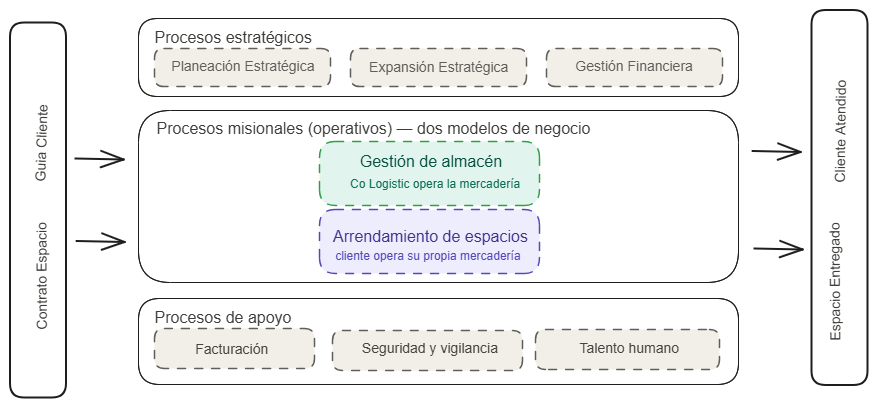
\includegraphics[width=0.95\textwidth]{./images/MAPA DE PROCESOS NIVEL 0.png}
  \caption{Extracto de la Matriz de Procesos Estratégicos}
\end{figure}

\vspace{1.5em}

\begin{center}
  \small
  \begin{tabularx}{\textwidth}{>{\centering\arraybackslash}X >{\centering\arraybackslash}X >{\centering\arraybackslash}X >{\centering\arraybackslash}X >{\centering\arraybackslash}X}
  \toprule
  \textbf{S} & \textbf{I} & \textbf{P} & \textbf{O} & \textbf{C} \\
  \textbf{Proveedores (del Proceso)} & \textbf{Elementos de entrada} & \textbf{Proceso} & \textbf{Productos (Elementos de Salida)} & \textbf{Clientes (del Proceso)} \\
  \midrule
  \textit{Gerente General /Subgerencia / Operaciones} & \textit{Información del entorno (político, económico, normativo)} & \textit{Diagnóstico estratégico organizacional} & \textit{Matriz FODA aprobada formalmente y diagnóstico interno/externo consolidado} & \textit{Jefatura de TI y Área de Gestión y Gobierno TI} \\
  \midrule
  \textit{Jefatura de TI y Estratega de Gobierno TI} & \textit{Matriz FODA aprobada formalmente y diagnóstico interno/externo consolidado} & \textit{Definición de la dirección estratégica} & \textit{Misión, visión, objetivos estratégicos y portafolio priorizado de iniciativas estratégicas aprobado} & \textit{Director de Proyectos TI} \\
  \midrule
  \textit{Director de Proyectos TI (PMO) y Área de Gestión y Gobierno TI} & \textit{Misión, visión, objetivos estratégicos y portafolio priorizado de iniciativas estratégicas aprobado} & \textit{Formulación del plan estratégico} & \textit{Plan estratégico y de acción formalizado como documento oficial} & \textit{Comité Gerencial y Gerente General} \\
  \midrule
  \textit{Jefatura de TI} & \textit{Plan estratégico y de acción formalizado como documento oficial} & \textit{Comunicación y alineamiento organizacional} & \textit{Fichas de alineamiento estratégico (compromisos por área)} & \textit{Jefaturas/Área de Gestión y Gobierno TI} \\
  \midrule
  \textit{Jefaturas/ Área de Gestión y Gobierno TI} & \textit{Fichas de alineamiento estratégico (compromisos por área),} & \textit{Seguimiento, control y revisión estratégica} & \textit{Reportes de avance de KPIs, actas de revisión estratégica e insumos actualizados} & \textit{Gerente General/jefatura de TI} \\
  \bottomrule
  \end{tabularx}
\end{center}

\vspace{7em}


\begin{center}
  \small
  \begin{tabularx}{\textwidth}{p{0.15\textwidth}p{0.18\textwidth}XXp{0.25\textwidth}}
  \toprule
  \multicolumn{2}{c}{\textbf{Macro Proceso}} & \multicolumn{2}{c}{\textbf{Proceso}} & \multirow{2}{*}{\textbf{Procedimientos}} \\
  \cmidrule(r){1-2} \cmidrule(l){3-4}
  \textbf{Título} & \textbf{Líder} & \textbf{Título} & \textbf{Líder} & \\
  \midrule
  Gestión de planeación estratégica & Gerente/ Area de TI & Gestión de planeación estratégica & Gerente/ Area de TI & 
  \begin{itemize} 
    \item Diagnóstico estratégico organizacional 
    \item Definición de la dirección estratégica 
    \item Formulación de plan estratégico 
    \item Comunicación y alineamiento organizacional 
    \item Seguimiento, control y revisión estratégica 
  \end{itemize} \\
  \bottomrule
  \end{tabularx}
\end{center}

\newpage

% ==========================================
\chapter{Procedimientos}
% ==========================================

% ------------------------------------------
\section{gestión de planeación Estrategica}
% ------------------------------------------
\textbf{Líder:} Gerencia General

\textbf{Participantes:}
\begin{itemize}
  \item Gerencia General
  \item Subgerencia
  \item Contador
  \item Jefe de Operaciones
  \item Analista 
  \item Personal Operativo
  
\end{itemize}

\textbf{Descripción del Procedimiento:} \\
Gestión de Planeación Estratégica es el proceso directivo fundamental encargado de analizar, trazar y controlar la ruta de crecimiento a largo plazo de la empresa. A diferencia de un plan tecnológico, este proceso parte de un diagnóstico interno y externo para entender la capacidad de la infraestructura física (40,000 m²), la competencia y los riesgos del entorno
. Su propósito central es transformar el modelo de negocio: pasar de ser una empresa que solo alquila metros cuadrados ("arrendamiento") a convertirse en un operador logístico integral.



%%%
\begin{center}
  \small
  \begin{tabularx}{\textwidth}{>{\raggedright\arraybackslash}p{0.15\textwidth} >{\raggedright\arraybackslash}p{0.18\textwidth} >{\raggedright\arraybackslash}X >{\raggedright\arraybackslash}p{0.18\textwidth} >{\raggedright\arraybackslash}p{0.15\textwidth}}
  \toprule
  \textbf{S} & \textbf{I} & \textbf{P} & \textbf{O} & \textbf{C} \\
  \textbf{Proveedores} & \textbf{Elementos de Entrada} & \textbf{Proceso / Actividades} & \textbf{Elementos de Salida} & \textbf{Clientes} \\
  \midrule
  Gerente General /Subgerencia / Operaciones & Información del entorno (político, económico, normativo) & Diagnóstico estratégico organizacional & Matriz FODA aprobada formalmente y diagnóstico interno/externo consolidado & Jefatura de TI y Área de Gestión y Gobierno TI \\
  \midrule
  Jefatura de TI y Estratega de Gobierno TI & Matriz FODA aprobada formalmente y diagnóstico interno/externo consolidado & Definición de la dirección estratégica & Misión, visión, objetivos estratégicos y portafolio priorizado de iniciativas estratégicas aprobado & Director de Proyectos TI \\
  \midrule
  Director de Proyectos TI (PMO) y Área de Gestión y Gobierno TI & Misión, visión, objetivos estratégicos y portafolio priorizado de iniciativas estratégicas aprobado & Formulación del plan estratégico & Plan estratégico y de acción formalizado como documento oficial & Comité Gerencial y Gerente General \\
  \midrule
  Jefatura de TI & Plan estratégico y de acción formalizado como documento oficial & Comunicación y alineamiento organizacional & Fichas de alineamiento estratégico (compromisos por área) & Jefaturas/Área de Gestión y Gobierno TI \\
  \midrule
  Jefaturas/ Área de Gestión y Gobierno TI & Fichas de alineamiento estratégico (compromisos por área), & Seguimiento, control y revisión estratégica & Reportes de avance de KPIs, actas de revisión estratégica e insumos actualizados & Gerente General/jefatura de TI \\
  \bottomrule
  \end{tabularx}
\end{center}

\vspace{1em}

\begin{figure}[h!]
  \centering
  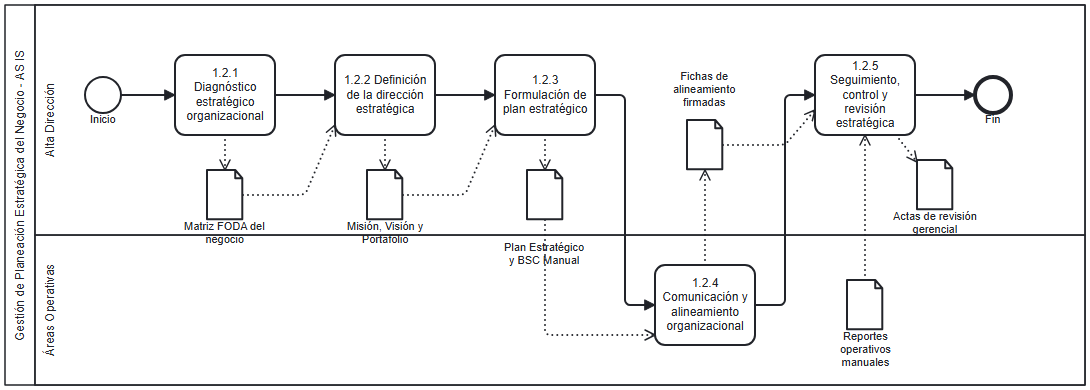
\includegraphics[width=1\textwidth]{./images/GPE_general.png}
  \caption{Diagrama de Procesos con BPMN - Gestión de planeación Estrategica}
\end{figure}

\newpage


% ==========================================
\chapter{Matriz de Indicadores}
% ==========================================
\newpage

\fichaIndicador{1. Diagnóstico Estratégico Organizacional}{Tasa de análisis de variables del entorno}{Medir la exhaustividad en el análisis de las variables críticas externas e internas identificadas en el diagnóstico}{(Número de variables críticas analizadas / Total de variables clave del entorno identificadas) $\times$ 100}{GPE\_001}{Gerencia General}{Subgerente}{100\%}{Anual}

\fichaIndicador{2. Definición de la Dirección Estratégica}{Índice de consenso de los pilares estratégicos}{Medir el nivel de acuerdo e institucionalización de la misión, visión, valores y portafolio de iniciativas prioritarias}{(Número de directores alineados y conformes con la propuesta / Total de miembros del comité de dirección general) $\times$ 100}{GPE\_002}{Gerencia General}{Subgerente}{100\%}{Anual}

\fichaIndicador{3. Formulación del Plan Estratégico}{Nivel de formalización y costeo de iniciativas}{Monitorear el avance en la especificación y asignación presupuestaria de los proyectos prioritarios para la transición a operador 3PL}{(Número de iniciativas estratégicas formalizadas y costeadas / Total de iniciativas definidas en el plan) $\times$ 100}{GPE\_003}{Gerencia General}{Subgerente}{100\%}{Anual}

\fichaIndicador{4. Comunicación y Alineamiento Organizacional}{Tasa de suscripción de compromisos estratégicos}{Garantizar que todas las áreas operativas clave suscriban sus correspondientes fichas de compromiso y alineamiento}{(Número de áreas operativas con fichas de compromiso firmadas / Total de áreas operativas clave de la empresa) $\times$ 100}{GPE\_004}{Subgerente}{Jefaturas de Área}{100\%}{Anual}

\fichaIndicador{5. Seguimiento, Control y Revisión Estratégica}{Cumplimiento de reuniones de revisión de la estrategia (BSC)}{Monitorear la regularidad de las revisiones del Balanced Scorecard para tomar decisiones tácticas oportunas}{(Número de sesiones de revisión estratégica ejecutadas con actas de conformidad / Total de sesiones planificadas en el año) $\times$ 100}{GPE\_005}{Gerencia General}{Subgerente}{100\%}{Trimestral}

\fichaIndicador{6. Gestión de la Planeación Estratégica General}{Eficacia global en la ejecución del Balanced Scorecard}{Medir el porcentaje de avance general ponderado en el cumplimiento de los hitos y metas anuales del BSC}{Sumatoria del porcentaje de avance de cada iniciativa del BSC / Total de iniciativas estratégicas del plan}{GPE\_006}{Gerencia General}{Subgerente}{$\ge$ 85\%}{Semestral}

\newpage

% ==========================================
\chapter{Documentos Generados}
% ==========================================

\begin{tabularx}{\textwidth}{>{\raggedright\arraybackslash}X >{\raggedright\arraybackslash}p{0.15\textwidth} >{\raggedright\arraybackslash}p{0.18\textwidth} >{\raggedright\arraybackslash}X}
\toprule
\multirow{2}{*}{\textbf{DOCUMENTO (QUÉ)}} & \multicolumn{3}{c}{\textbf{CUSTODIA}} \\
\cmidrule{2-4}
& \textbf{QUIÉN} & \textbf{DÓNDE} & \textbf{CÓMO} \\
\midrule
Matriz FODA del negocio & Subgerente & Carpeta digital compartida & Archivo en formato PDF o Excel consolidado tras los talleres de diagnóstico \\
\midrule
Reporte de entorno (interno/externo) & Subgerente & Carpeta digital compartida & Documento de diagnóstico con análisis político, económico y de mercado \\
\midrule
Declaración de Misión, Visión y Valores & Gerente General & Intranet / Carpeta institucional & Documento formal PDF aprobado por el comité directivo \\
\midrule
Portafolio de iniciativas prioritarias & Subgerente & Hoja de cálculo en la nube & Consolidado de proyectos clave para la transición a operador 3PL \\
\midrule
Plan Estratégico General & Gerente General & Carpeta digital / Archivador físico & Documento oficial en PDF con firmas del comité directivo \\
\midrule
Balanced Scorecard (BSC Manual) & Subgerente & Hoja de cálculo en la nube & Matriz en Excel que detalla objetivos, KPIs, metas y responsables \\
\midrule
Fichas de alineamiento estratégico por área & Subgerente & Carpeta compartida de control & Escaneado de fichas impresas firmadas por los jefes de área de forma física o digital \\
\midrule
Reportes operativos de avance de KPIs & Jefaturas de Área & Correo electrónico / Carpeta compartida & Archivos Excel enviados periódicamente como insumo para el BSC \\
\midrule
Actas de revisión estratégica gerencial & Gerente General & Archivador físico / Carpeta digital & Documento firmado con los compromisos y ajustes estratégicos decididos \\
\bottomrule
\end{tabularx}

\vspace{2em}

% ==========================================
\chapter{Anexos}
% ==========================================
\textbf{ANEXO N° 01:} [Título del Anexo] \\
\textbf{ANEXO N° 02:} [Título del Anexo]

\end{document}
